\subsection{Research Objectives and Anticipated Results}

%\begin{wrapfigure}{l}{0.62\textwidth}
%\begin{figure}[t]
%    \centering
%    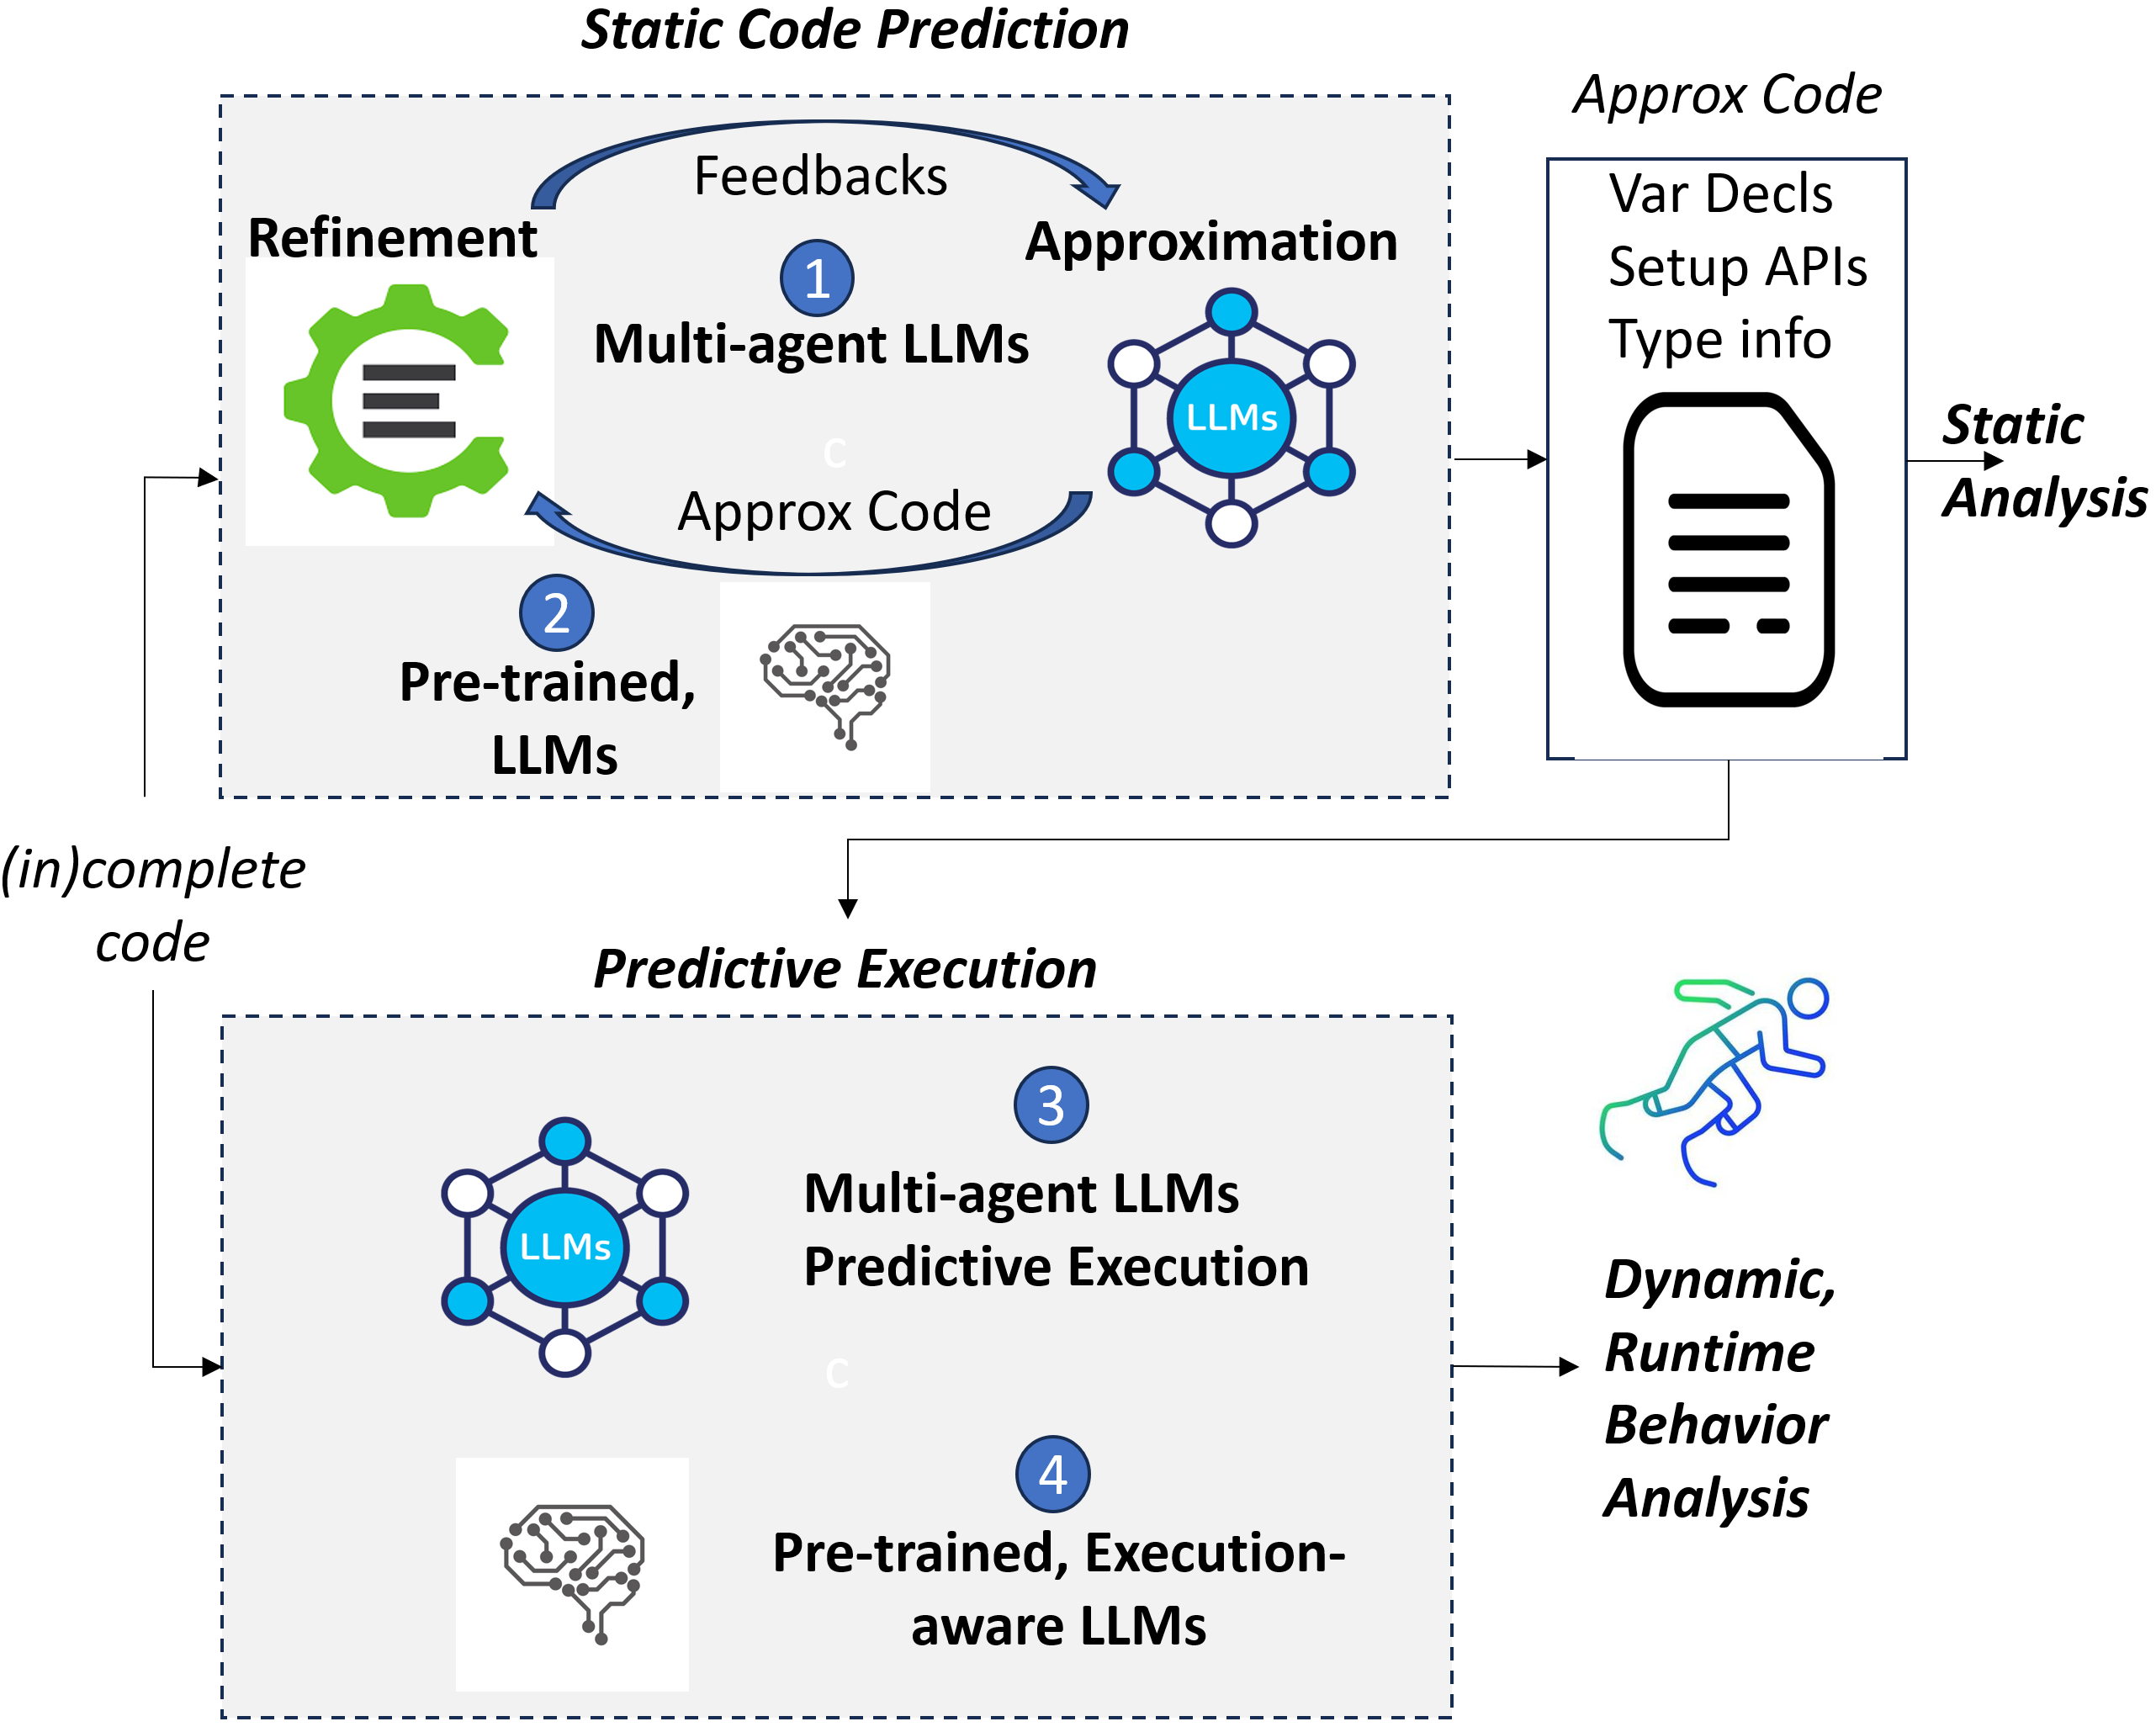
\includegraphics[width=0.62\textwidth]{overview-new.png}
%    \vspace{-10pt}
%    \caption{Predictive Program Analysis: Analyzing Dynamic Program Behaviors}
%    \label{fig:arch}
%\end{wrapfigure}


We seek to advance the state-of-the-art in fuzz testing by means of
{\tool}, a {\bf Predictive Coverage-Guided Intelligent Fuzzing}
framework, with the goal of overcoming the issues listed in the
introduction. We aim to establish {\em a scientific foundation, novel
  methodologies, frameworks, models, and algorithmic solutions for
  predictive coverage-guided fuzz testing} with the following focus
areas:



(1) Large Language Models (LLM)-based {\bf predictive code coverage} (without test execution),

(2) LLM-based, targeting, {\bf test case generation}, and

(3) {\bf predictive coverage-guided fuzz testing} with LLMs.

%\noindent Figure~\ref{fig:arch} illustrates the framework for {\tool},
%which will allow the construction of efficient program analysis
%techniques for (partial) code, also based on which downstream vulnerability detection and assessment applications can be built.

Our predictive program analysis framework is also beneficial in other
scenarios in addition to programming assistants for incomplete code in
an IDE. Predictive execution is not aimed to replace actual
execution. Rather, it offers a solution where the actual execution is
impossible, specifically in the scenarios 1) where the complete source
code is not available, or 2) where the analysis or approximation on
the behavior of the code is needed/desired without actual execution
and some degree of inaccuracy in prediction is tolerable.  First, the
first scenario can be exhibited in several examples, e.g., in the code
snippets in Stack Overflow or GitHub gist. They often miss contextual
information, such as imports and definitions of variables and
functions. It can take a great deal of efforts to integrate such code
snippets to a codebase.
%Horton and Parnin~\cite{horton2018gistable} reported that ``75.6\% of
%Python code snippets in gist require non-trivial configuration to
%overcome missing dependencies, configuration files, reliance on a
%specific operating system, or some other environment
%configuration''. Hossain {\em et al}~\cite{hossain2019executability}
%found that after installing the top 40~Python packages, the overall
%execution success rate for Stack Overflow Python code snippets is only
%27.9\% considering those running in either Python 2 or Python 3
%environments.
%Moreover, in~his keynote,
%Yahav~\cite{yahav2023fse} poses a need to approximate the execution of
%the incomplete code under editing in an AI-assisted programming
%environment.
Second, the instances of the second scenario can include the
analysis/approximation~of the behavior to check properties of
untrusted code or~to~detect bugs early. Moreover, even with complete
code, setting~up running environments for dynamic analysis is
undesired due to missing third-party dependencies and complex build
configurations.

The \underline{key philosophy} that drives our work is that the analysis of
partial code can be learned from the analysis of entire programs in
the wealth of information obtained from ultra-large-scale, open-source
software repositories. To accomplish these tasks, we propose the
following thrusts of research in {\tool} (Figure~\ref{fig:arch}):

\noindent \textbf{Thrust 1. LLM Multi-agents and Pre-trained Language Models for Static Analysis on Incomplete Code.} ({\em Section~\ref{sec:thrust1}})
As depicted in Figure~\ref{fig:pre-rec}, conventional Program Analysis
(PA) techniques exhibit high precision and recall when applied to
complete code. However, when dealing with incomplete code, these
techniques may experience a significant decrease in recall due to
missing information, despite maintaining reasonably high precision or
experiencing a slight decrease in precision due to their strict and/or
heuristic analysis rules (denoted by PA $\medblacklozenge$ in
Figure~\ref{fig:pre-rec}). On the other hand, employing an LLM directly
for downstream analysis tasks may yield higher recall, thanks to the
LLM's ability to explore the solution space (denoted by LLM
$\circledast$ in Figure~\ref{fig:pre-rec}). However, the precision of
  LLM analysis on incomplete code tends to be lower compared to
  conventional PA tools due to the lack of ability in specific
  analysis in the downstream tasks.

We propose a tandem solution that combines LLMs and PA agents to
leverage the strengths of both methodologies. We aim to harnessing the
complementary capabilities of LLMs and PA: {\em LLMs' expansive search
  capabilities} and {\em PA-based agents' semantic verification
  abilities}.
%This integrated approach aims to optimize performance by
%harnessing the complementary capabilities of LLMs and PA
%techniques.

We advocate for a novel paradigm, called {\bf predictive program
  analysis}, which operates on the principles of {\em
  Approximation-Refinement} for Analysis. In the Approximation phase,
a large language model (LLM) acts as a machine learning (ML) agent to
fill in missing information within incomplete code. The missing
information that will be filled by the LLM could be manifested {\em
  explicitly}, e.g., in terms of missing variable declarations, setup
API method calls, import statements, and exception handling types, or
{\em implicitly}, e.g., in terms of missing type information of 
program elements, missing dependencies, etc.

%Leveraging an LLM for this is advantageous due to its capability of code understanding.

\begin{wrapfigure}{l}{0.55\textwidth}
    \centering
    \begin{tikzpicture}
        \pgfplotsset{width=3in,
         }
        \begin{axis}[
            scale=1,
            view={20}{35},
            ticklabel style={font=\footnotesize},
            xlabel={\normalsize \textbf{Precision} ($\rightarrow$)},
            ylabel={\normalsize \textbf{Recall} ($\rightarrow$)},
%            zlabel={\normalsize \textbf{Source Code} ($\rightarrow$)},
            xlabel style={rotate=-10, yshift=0.1cm},
            ylabel style={yshift=0.5cm, xshift=0.225cm,rotate=65},
            zlabel style={yshift=-0.2cm, xshift=-0.5cm,rotate=0},
            xmin=0, xmax=4,
            xtick={1,2,3},
            ymin=0, ymax=4,
            ytick={1,2,3},
            zmin=0, zmax=1,
            ztick={0,1},
            xticklabels={\textit{Low},\textit{Medium},\textit{High}}, % Set custom x-tick labels
            yticklabels={\textit{Low},\textit{Medium},\textit{High}}, % Set custom y-tick labels
            zticklabels={\textit{Partial Code},\textit{Complete Code}},
            ztick pos = left,
            xticklabel style={rotate=0},
            yticklabel style={rotate=0, yshift=0.325cm},
            zticklabel style={yshift=0.4cm},
            % Set custom z-tick labels
            axis background/.style={fill=gray!10},
            xmajorgrids=true,
            ymajorgrids=true,
            zmajorgrids=true,
            grid style={dotted, thick},
            axis equal,
            visualization depends on={value \thisrow{m} \as \labela},
        ]
        % Add a node at x=High, y=High, z=Complete
        \draw[dashed,black,thick] (axis cs:3,3,1) -- (axis cs:0,3,1) node[midway, right] {};
        \draw[dashed,black,thick] (axis cs:3,3,1) -- (axis cs:3,4,1) node[midway, below] {};
        \draw[dashed,black,thick] (axis cs:3,3,1) -- (axis cs:3,3,-0.2);
        \node[above right] at (axis cs:{2.9,2.55,1}) {\textcolor{blue}{\large $\medblacklozenge$}};

        % Thick axes
        \draw[black, thick] (axis cs:0,4,-0.3) -- (axis cs:4,4,-0.3) node[midway, right] {};
        \draw[black, thick] (axis cs:0,4,-0.3) -- (axis cs:0,0,-0.3) node[midway, right] {};
        \draw[black, thick] (axis cs:0,4,-0.3) -- (axis cs:0,4,1.3) node[midway, right] {};
        

        % Add points.
        \node[above right] at (axis cs:{3,0.75,0}) {\textcolor{red}{\large $\medblacklozenge$}};
        \node[above right] at (axis cs:{2.95,1.85,0}) {{\textcolor{meatbrown}{\small $\bigstar$}}};
        \node[above right] at (axis cs:{2.55,1.5,0}) {\textcolor{red}{{\small $\circledast$}}};

        % % Add Origin
        % \node[above right] at (axis cs:{4,-0.2,0}) { $\circ$};

        % Add optimal point
        \node[above right] at (axis cs:{3.08,2.3,0}) { \textcolor{dkgreen}{{\footnotesize $\circ$}}};

        \end{axis}
        \draw[gray,line width=0.5pt,rotate=15,fill=red,opacity=0.125] (3.75,0.85,0) circle (1.75 and 0.85);

        % Add node labels
        \node[text width=2cm] at (6,3.75,1) 
            {\footnotesize{\textcolor{blue}{PA}}};
        \node[text width=2cm] at (5.0,1.275,0) 
            {\footnotesize{\textcolor{red}{PA}}};
        \node[text width=2cm] at (4,2.025,0) 
            {\footnotesize{\textcolor{red}{LLM+PA}}};
         \node[text width=2cm] at (3.875,1.7,0) 
            {\footnotesize{\textcolor{red}{LLM}}};
    \end{tikzpicture}
    \vspace{-20pt}
    \caption{Efficacy of various \textcolor{red}{\textit{\textbf{partial}}} and \textcolor{blue}{\textit{\textbf{complete}}} program analysis approaches, with ({\small $\medblacklozenge$}), and without ({\footnotesize $\circledast$}, {\footnotesize $\bigstar$}) learning-based knowledge.}
    \label{fig:pre-rec}
\end{wrapfigure}


A naive solution is to take whatever information the LLMs completed
and feed to a traditional program analysis as is. However,
researchers have shown that while LLMs are remarkable in code
generation with correct syntaxes, the produced code often contains
semantic errors and even do not compilable.  Thus, the Refinement
phase employs a program analysis (PA)-based agent to verify the
completed code output by the LLM. This PA-based agent utilizes the
compiler technology to ensure that the generated code is compilable
and consistent with used external libraries. The iterative interplay
between the LLM-based agent and the PA-based agent continues until a
compilable code is achieved.
%If after a specified number of iterations the code remains
%uncompilable, human intervention may be sought for final resolution.
In brief, the interplay between LLM and PA agents has two objectives:
1) to enhance recall compared to the PA-only solution (via the
Approximation of the incomplete code), and 2) to
maintain or even improve precision beyond what can be achieved with
LLM-only solution by integrating PA to ``correct'' the LLM's solution
(via the result Refinement).
%{\em Such interplay between the LLM and PA agents aims to enhance both the
%recall and precision} of the analysis when comparing with the approach
%using directly the PA technique on the incomplete code.

%The LLM is used to expand the candidate list of potential complete
%code for the current incomplete snippet, and PA is used to verify to
%make sure the validity of the chosen candidate. Subsequently,
%downstream program analysis techniques can be applied in the Analysis
%phase.
%It's important to acknowledge that the LLM may not always be capable
%of providing the exact missing information that developers would
%create when incorporating incomplete code snippets into their projects
%because each project might have its own . However, leveraging its
%proficiency in understanding code, we anticipate that it will fill in
%the gaps with the most probable information for the given incomplete
%code. Subsequently, following verification by the PA agent, the code
%is rendered complete and ready for analysis techniques to generate
%more accurate results in which without our framework, these techniques
%would be ineffective in handling incomplete code.







%One of the key foundations of {\tool} lies in its neural structural analysis component, which is built upon the well-defined structure and semantics of source code. This component serves two primary functions. Firstly, it draws upon the syntactic structures of comprehensive code samples from large-scale repositories in the training dataset. From this data, it constructs an abstract syntax tree (AST) that best encapsulates the syntactic arrangement of the provided partial code, aiming for the highest likelihood or probability. In contrast, existing program-analysis-based partial parsing methods~\cite{ppa08} rely on heuristics derived from the syntactic rules of programming languages, lacking the capacity to rank or score potential candidates. The second task of this component involves labeling code tokens with the corresponding types of syntactic units, encompassing statement types (\code{if}, \code{for}, etc.), variables, fields, methods, classes, and more. Both tasks can be efficiently executed through our dual-learning-based approaches.

%Source code has a well-defined structure and semantics. Thus, the basic infrastructure in {\tool} is the neural structural analysis component, which primarily has two tasks. First, it learns from the syntactic structures of the complete code in the training dataset collected from large-scale code repositories, to derive the abstract syntax tree (AST) that best represents the syntactic structure of the given partial code, i.e., with the highest likelihood/probability. The existing program-analysis-based partial parsing approaches~\cite{ppa08} rely on the heuristics on the syntactic rules of the programming languages. They do not give us any ranking or scores among the potential candidates. The second task of this component is to tag the code tokens with the types of the syntactic units including the statement types (\code{if}, \code{for}, etc.), variables, fields, methods, classes, etc. Both of the tasks can be performed with our learning-based approaches in a dual-learning manner.
  
%\vspace{3pt}
%\noindent \textbf{Thrust 2. Pre-trained Large Language Models for
%  Incomplete Code Static Analysis} ({\em Section~\ref{sec:thrust2}})
%Our work is driven by the fundamental belief that insights gained from
%training by complete programs within vast repositories of
%ultra-large-scale, open-source software can inform the analysis of
%partial code.

While exploring LLM-based multi-agent solution, we also aim to develop
smaller models via pre-trained language models. Our work is driven by
the fundamental belief that insights gained from training by complete
programs within vast repositories of ultra-large-scale, open-source
software can inform the analysis of partial code~\cite{naturalness-icse12}.
%Hindle {\em et al.}~\cite{naturalness-icse12} have shown that code has
%high repetitiveness and predictability and can be captured well by
%statistical models.
Thus, we expect to build/fine-tune pre-trained LLM models to learn
from those repositories.



%The basis components for several analysis techniques on the semantics
%of the program could tentatively include the following (more
%components will be added as the project evolves):

%1) the identification of the APIs of the external libraries in the
%external references in the partial code: this is needed because the
%partial code contains the undeclared reference and/or
%declaration/reference ambiguity without explicit declaration of the
%APIs in the external libraries. The knowledge on the external
%libraries enables more precise analysis of the code snippets.

%2) the inference of the type information for the entities in the
%partial code: due to the ambiguity in the declaration, the types of
%the variables and statements are not always obviously
%identified. Thus, the type inference is a basic service within
%{\tool}.

%3) the inference of the program dependencies among the statements in
%the partial code: several program analysis techniques are based on the
%program dependencies, which are not always obtainable due to the
%incompleteness of the given code fragment.

%4) Program slicing: program slices are important in both code
%understanding and program analysis for code snippets. That allows the
%analysis on the statements affecting or to be affected by a specified
%variable. All traditional program slicing techniques require the code
%to be complete.

\vspace{3pt}
\noindent \textbf{Thrust 2. LLM Multi-agents and Pre-trained
  Language Models for Predictive Execution.}  ({\em
  Section~\ref{sec:thrust2}})

We advocate for an execution paradigm called predictive execution. In
predictive execution, with a specific input, the execution is not
carried out with the computer performing the instruction in the
program. Instead, a trained machine learning model predicts the
execution steps and as a result, the execution trace corresponding to
the input is derived without actual execution.

By simulating program behaviors and outcomes without running the code,
these approaches provide valuable insights into the program's
potential runtime characteristics. Here are some benefits of
predictive execution. First, early error detection: predicting program
executions allows for the early detection of errors and potential
vulnerabilities before executing the code. By simulating different
execution paths and scenarios, predictive execution can enable the
dynamic analysis tools to identify potential issues such as null
pointer dereferences, memory leaks, or buffer overflows without the
need to execute the code in a real-world environment. This early error
detection helps developers catch and fix bugs more efficiently,
reducing the likelihood of critical issues in production. Second,
dynamic analysis techniques that predict program executions play a
crucial role in security analysis. By simulating potential attack
scenarios and analyzing how the program behaves under different
conditions, these tools can identify security vulnerabilities such as
injection attacks, privilege escalation, or data breaches. Predictive
execution helps security professionals assess the resilience
of systems against various threats and vulnerabilities,
enabling proactive security measures and robust defenses. Finally,
predicting executions provides developers with a deeper understanding
of their code's behavior without the need for actual execution. By
simulating program flows and interactions, tools can uncover hidden
dependencies, identify unexpected behaviors, and reveal complex
program dynamics.

%This insight into program behavior helps developers better comprehend their code, debug more effectively, and make informed design decisions.

In addition multi-agent solutions, we also explore the
pre-training language models. We aim to teach a smaller model to analyze
the runtime behaviors via the learning from complete programs in execution.


%Symbolic execution is a means of analyzing a program to determine what
%inputs cause each part of a program to execute. Symbolic execution
%performs executing a program abstractly, so that one abstract
%execution covers multiple possible inputs, which are assumed to have
%symbolic values. We aim to explore the novel area in AI named
%neuro-symbolic learning, which seeks to combine traditional
%rules-based AI approaches with modern deep learning techniques.  We
%will leverage traditional program analysis rules to enhance the
%learning of the characteristics on the execution of the partial code
%fragment.

\vspace{3pt}
\noindent \textbf{Thrust 3. Programming Assistant Applications with Predictive Program Analysis.}  ({\em Section~\ref{sec:thrust3}})


Our last thrust of research is aimed to demonstrate the usefulness of
our solution in different programming assistant applications: 1)
vulnerability detection, 2) dynamic slicing,  etc.

%and 3) debugging and error detection.



%2) fault localization, and 3) code completion.

%\vspace{3pt}
%\noindent \textbf{Thrust ???. Neural Execution Analysis Infrastructure.}
%({\em Section~\ref{}}) All the dynamic analysis techniques require the
%analysis and understanding of the execution. However, for an
%incomplete code, we first need to design a component that can wrap
%around the given code fragment with the minimum code so that the code
%fragment can be executed. When the code is executed, we also need the
%approaches that represent the executed statements and their relations,
%model the execution and stack traces, and model the code coverages
%for an execution.




%Toward this theme, in our preliminary work, we developed DeepPDA
%(Section~\ref{sec:deeppda}), a neural network-based partial program
%dependence analysis approach that learns to derive the program
%dependencies for any code fragments (i.e., both complete and
%incomplete). In our preliminary empirical evaluation, we intrinsically
%evaluated it on Java and C/C++ programs. We trained DeepPDA on
%complete code. For testing, we treated each method individually and
%chose a consecutive portion within the method to predict the program
%dependencies, and compared them against the actual
%dependencies. Overall, DeepPDA predicts CFGs/PDGs in Java with
%an F-score of 94.29\%, and in C++ with an F-score of 92.46\%. As
%another preliminary work (Section~\ref{sec:statype}), we also
%developed an approach to derive the data types of the variables in the
%code snippets. We treat the problem as statistical machine translation
%from source code with partially qualified names to source code with
%full names. Our preliminary evaluation on StackOverflow posts shows
%that our technique achieves high accuracy with 97.6\% precision and
%96.7\% recall in deriving data types in code snippets.

%We also test the usefulness of the PDGs predicted by DeepPDA (i.e.,
%PDG*) on the downstream task of method-level vulnerability
%detection. We discover that the performance of the vulnerability
%detection tool utilizing PDG* is only 1.1\% less than that utilizing
%the PDGs generated by a program analysis tool.
%We also report the detection of 14 real-world vulnerable code snippets
%from StackOverflow by a learning-based vulnerability detection
%tool that employs the PDGs predicted by DeepPDA for these code snippets.

\begin{table*}[t]
	\vspace{-15pt}
\begin{center}
{\footnotesize{
\begin{tabular}{cc}
\begin{tabular}[t]{|p{0.2in}|p{2.95in}|} 
\hline
\multicolumn{2}{|>{\columncolor[gray]{0}}c|}{\textcolor{white}
{\bf Year 1 Project Milestones \& Deliverables}}\\
\hline 
\hline
\multicolumn{2}{|c|}{\bf T1. LLM Multi-agents for Static Analysis}\\
\hline
{\bf 1.1} & LLM Multi-agent framework\\
{\bf 1.2} & LLM Multi-agent and Static Analysis\\
{\bf 1.3} & Pre-trained Language Models for Static Analysis\\
\hline
\hline
\multicolumn{2}{|c|}{\bf T1. Pre-trained Language Models for Static Analysis}\\ 
\hline
{\bf 1.4} & Pre-trained Language Models for Static Analysis\\
\hline
%\hline
%\multicolumn{2}{|c|}{\bf Integrate Code Synthesis into Tools}\\
%\hline
%{\bf 1.5} & \goalOneFour.\\
%\hline
\multicolumn{2}{c}{}
\end{tabular}
&
\begin{tabular}[t]{|p{0.2in}|p{2.95in}|} \hline
\multicolumn{2}{|>{\columncolor[gray]{0}}c|}{\textcolor{white}
{\bf Year 2 Project Milestones \& Deliverables}}\\
\hline 
\hline
\multicolumn{2}{|c|}{\bf T2. LLM Multi-agents for Predictive Execution}\\
\hline
{\bf 2.1} & LLM Multi-agents with Graphs\\
{\bf 2.2} & LLM Multi-agents with Execution\\
%{\bf 2.3} & Integrate Evaluation Framework into Design Environment\\
%{\bf 2.4} & Evaluate CRL Framework with Existing Models\\
%{\bf 2.3} & \goalTwoThree.\\

\hline
\hline
\multicolumn{2}{|c|}{\bf T2. Pre-trained Language Models for Predictive Execution}\\ 
\hline
%{\bf 3.1} & Design New Code Representations and Learning Models.\\
{\bf 2.3} &  Pre-trained Language Models for Predictive Execution\\
%{\bf 2.4} & Advance FL and RT-CI Approaches.\\
%{\bf 2.5} & Advance Regression Testing in CI Approaches.\\
%{\bf 2.5} & Advance APR Approaches with Framework.\\
\hline
%\hline
%\multicolumn{2}{|c|}{\bf Community Involvement: Capacity Building}\\
%\hline
%{\bf 2.4} & \goalTwoFour.\\
%{\bf 2.5} & \goalTwoFive.\\
%{\bf 2.6} & \goalTwoSix.\\
%\hline
\multicolumn{2}{c}{}
\end{tabular}
\end{tabular}\\
\vspace*{-.3cm}
\begin{tabular}{c}\hline
\multicolumn{1}{|>{\centering\columncolor[gray]{0}}p{6.44in}|}{\textcolor{white}
{\bf Year 3 Project Milestones \& Deliverables}}\\
\hline
\end{tabular}\\
\vspace*{-.2cm}
\begin{tabular}{cc}
\begin{tabular}[t]{|p{0.2in}|p{2.95in}|}
\hline
\multicolumn{2}{|c|}{\bf T3. Programming Assistant with Predictive Analysis}\\
\hline
{\bf 3.1} & Dependency Analysis\\
{\bf 3.2} & Debugging and Error Detection\\
\hline
%\hline
%\multicolumn{2}{|c|}{\bf \goalTwo}\\ 
%\hline
%{\bf 3.3} & \goalThreeThree.\\
%\hline
\multicolumn{2}{c}{}
\end{tabular}
&
\begin{tabular}[t]{|p{0.2in}|p{2.95in}|}
\hline
\multicolumn{2}{|c|}{\bf T3. Programming Assistant with Predictive Analysis}\\
\hline
%{\bf 3.1} & Design New Code Representations\\
{\bf 3.3} & Dynamic Slicing\\
\hline
\multicolumn{2}{c}{}
\end{tabular}
\end{tabular}
\vspace{-15pt}
}}
\end{center}
\vspace*{-.3in}
%\caption{Tasks and Milestones. (Rep. = Representation)}
\caption{The 3-year schedule of Thrusts, Tasks, and Milestones of this proposal.}
%the schedule of Thrusts, Tasks, and Milestones of this proposal.
%\vspace{-10pt}
\label{tab:milestones}
\vspace{-10pt}
\end{table*}
%

